\documentclass[10pt]{article}
\usepackage{amssymb,amsmath,times,url,graphicx,amsthm,alltt}
%\usepackage[pdftex,urlcolor=blue,pdfpagemode=none,pdfstartview=FitH]{hyperref}
\usepackage{my_packages}
\usepackage{tikz_packages}
%% url smaller font.
\makeatletter
\def\url@leostyle{%
  \@ifundefined{selectfont}{\def\UrlFont{\sf}}{\def\UrlFont{\small\ttfamily}}}
\makeatother
\urlstyle{leo}

%\usepackage[all,import]{xy}

\renewcommand{\baselinestretch}{1.2}
\date{}

\renewcommand{\thesubsection}{\arabic{subsection}. }
\renewcommand{\thesubsubsection}{\arabic{subsection}.\arabic{subsubsection} }

\theoremstyle{definition}
\newtheorem{prob}{Problem}[section]
%\renewcommand{\theprob}{\arabic{section}.\arabic{prob}}
\renewcommand{\theprob}{\arabic{prob}}

\newenvironment{subprob}%
{\renewcommand{\theenumi}{\alph{enumi}}\renewcommand{\labelenumi}{(\theenumi)}\begin{enumerate}}%
{\end{enumerate}}%

\newenvironment{matlab}
{\begin{alltt}\small\renewcommand{\baselinestretch}{1.2}\selectfont}%
{\end{alltt}}


\begin{document}

\pagestyle{empty}
\section*{MAE3145: Homework 2}
\vspace*{-0.4cm}
\noindent{Due date: September 13, 2017}%\\%\vspace*{0.5cm}

\begin{prob}
    The Juno spacecraft was launched August 5, 2011 and is now in orbit of Jupiter, having inserted into an highly elliptical Jovian orbit on July 5, 2016.
    Juno is the first deep-space vehicle to use solar panels at Juptier, as all previous missions have relied on radioisotope thermoelectric generators. 
    Furthermore, considereable effort has been expended in the design of the orbit of Juno in the Jovian system. 
    Due to the extreme distance, the orbit is chosen to provide nearly continuous solar illumination, and to avoid the intense radition environment of Jupiter.
    \begin{figure}[htbp]
        \centering
        \begin{subfigure}[htbp]{0.5\textwidth} 
            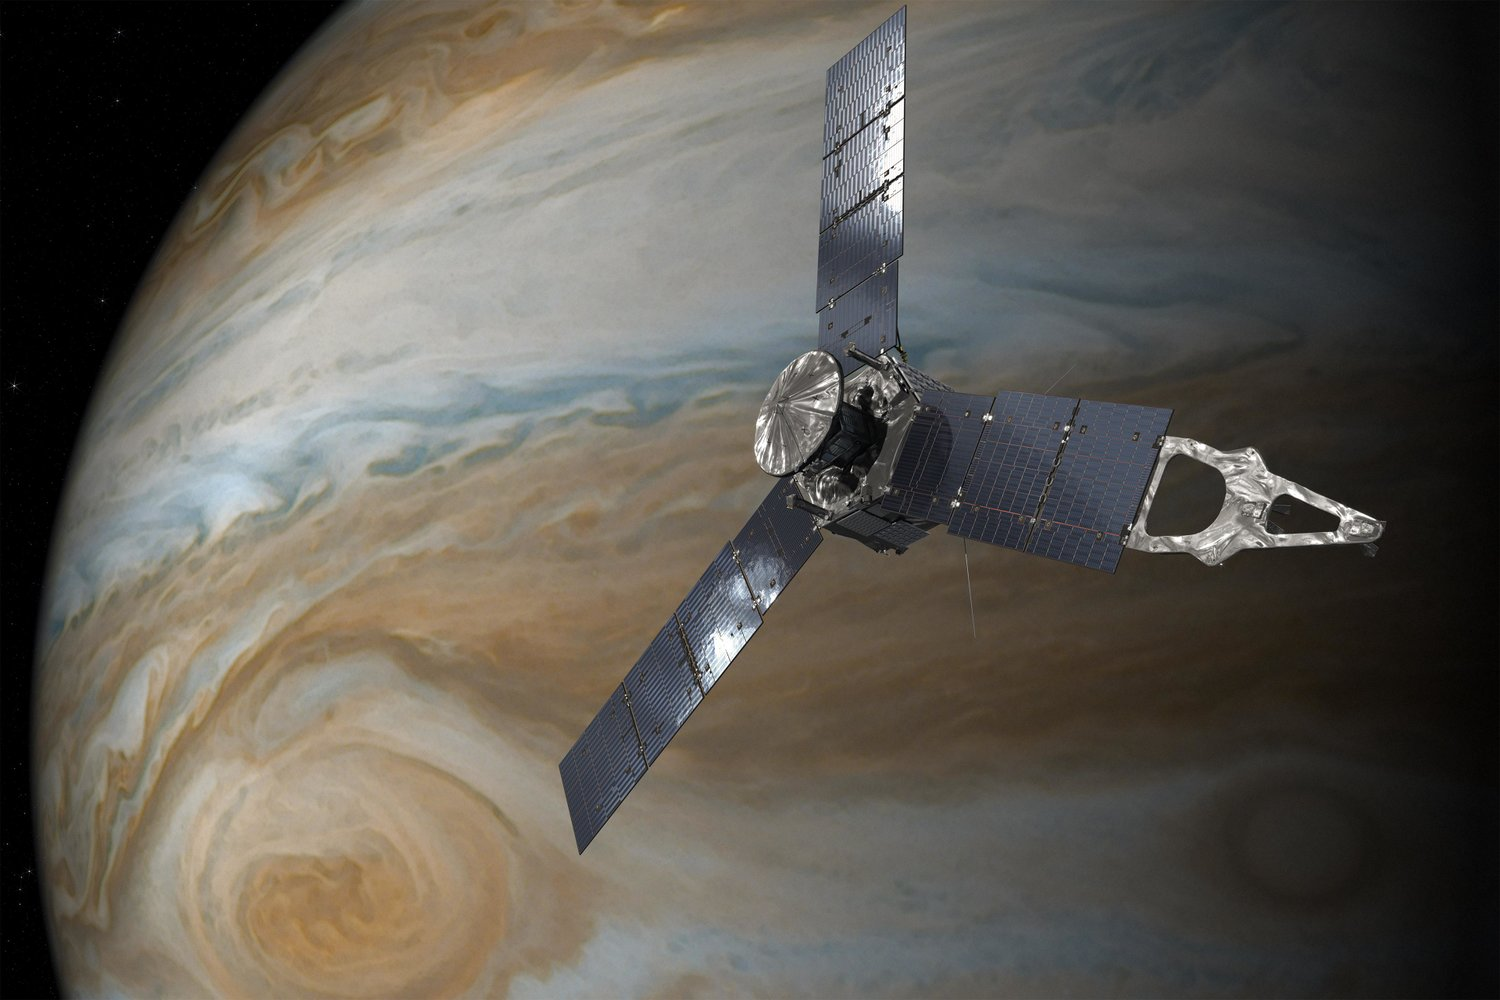
\includegraphics[width=\textwidth, keepaspectratio]{figures/juno.jpg} 
            \caption{Juno Spacecraft \label{fig:juno}} 
        \end{subfigure}~ 
        \begin{subfigure}[htbp]{0.5\textwidth} 
            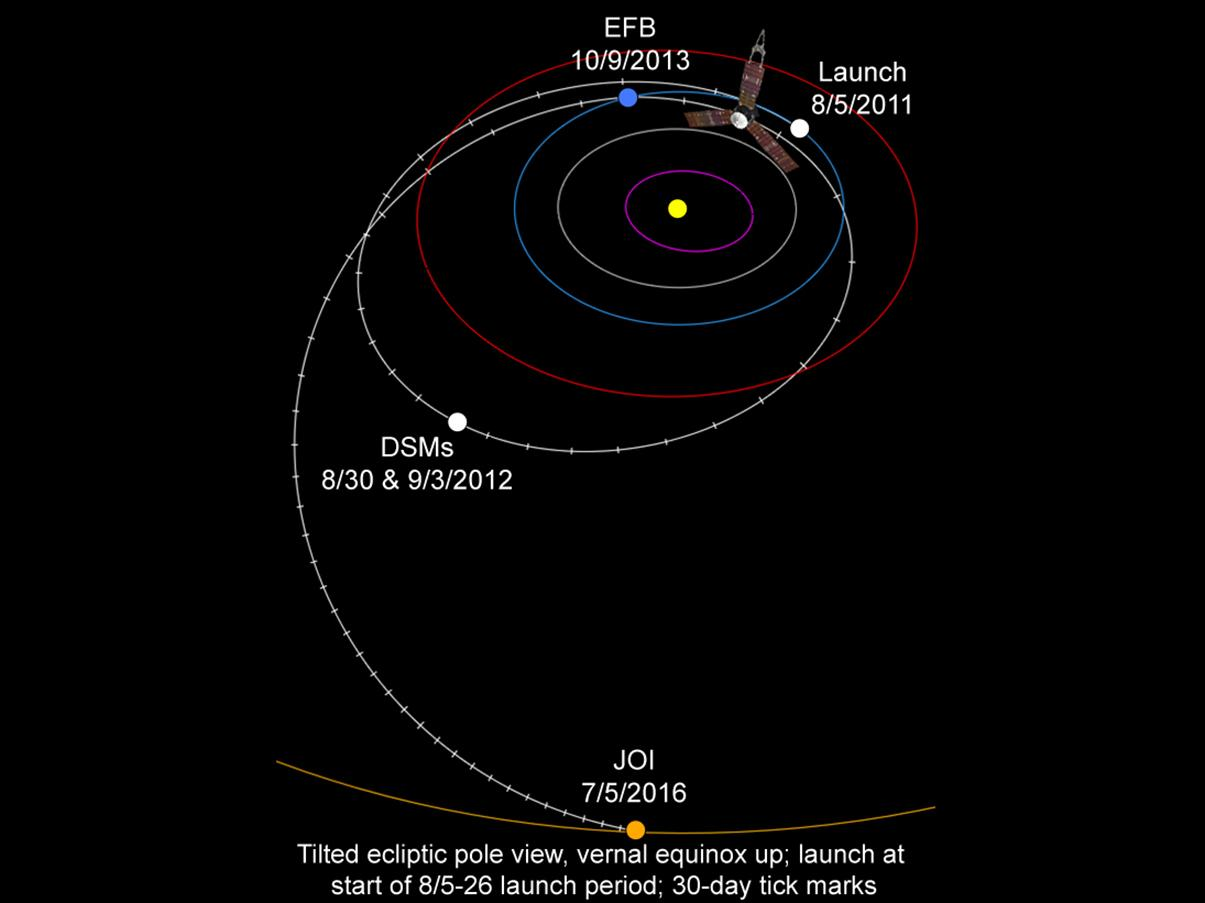
\includegraphics[width=\textwidth, keepaspectratio]{figures/trajectory.jpg} 
            \caption{Trajectory \label{fig:trajectory<`4`>}} 
        \end{subfigure} 
    \end{figure}
        
    After arriving in the Jovian system, Juno first entered a highly elliptical orbit which passed the orbit of the moon Callisto.
    Assume that during the first capture orbit the bodies are aligned as shown in~\cref{fig:planets}.
    \begin{figure}[htbp]
        \centering
        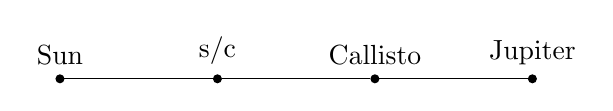
\begin{tikzpicture}
            [
            point/.style = {draw, circle, fill = black, inner sep = 1pt},
            dot/.style = {draw, circle, fill = black, inner sep = 0.2pt}
            ]
            % three corners of the triangle
            \node (s) at (0, 0) [point, label = {Sun}] {};
            \node (sc) at (2, 0) [point, label = {s/c}] {};
            \node (c) at (4, 0) [point, label = {Callisto}] {};
            \node (j) at (6, 0) [point, label = {Jupiter}] {};

            \draw (s) -- (sc) -- (c) -- (j);
        \end{tikzpicture}
        \caption{Planet alignment~\label{fig:planets}}
    \end{figure}
    
    Assume all bodies are in circular orbits with a radius equal to their semimajor axis. 
    A table of constants for some planetary moons has been provided on Blackboard.
    During orbit insertion, Juno passed within \textbf{\SI{4000}{\kilo\meter}} from the center of Callisto!

    \begin{subprob}
        \item At this instant, calculate the accelerations on the spacecraft with respect to Jupiter due to the gravity fields from the Sun, Callisto and Jupiter.
            Determine the dominant, direct, and indirect accelerations, including the directions. 

            Which one is the smallest? Largest? Is the dominant acceleration actually the largest?

        \item Determine the magnitude and direction of the perturbing accelerations. 
            Which body delivers the largest perturbing acceleration?
            For this alignment, consider each perturbning term. 
            Does the perturbing acceleration from the Sun tend to pull the spacecraft and Jupiter apart or drive the bodies together?
            What about the perturbation from Callisto?

        \item Given this four-body system, for the orbit of the spacecraft with respect to Jupiter, is a two-body orbit model sufficient to represent the path?
            If you had to decide to keep only one additional body in the model, would you keep the Sun or Callisto at this instant?
    \end{subprob}
    
    \begin{figure}[htbp]
        \centering
        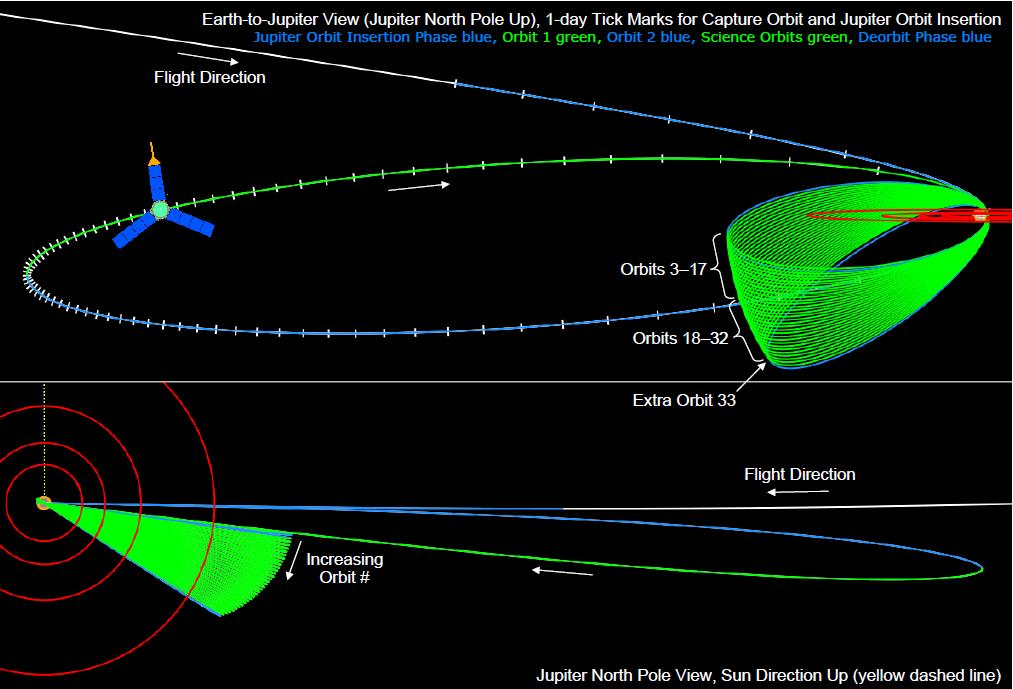
\includegraphics[width=\textwidth]{figures/jupiter_orbit.jpg}
        \caption{Juno orbits about Jupiter. The orbit plane is chosen to lie orthogonal to the Sun-Jupiter vector. In other words, the orbit angular momentum vector is designed such that it aligns with the direction to the Sun. This ensures that Juno is always illuminated and the polar orbits avoid the majority of the radiation environment at Jupiter.~\label{fig:jupiter_orbit}}
    \end{figure}
\end{prob}

\end{document}

